Im Gegensatz zum Konzept umfasst der Prototyp mehr Nutzerinteraktionen. Der 
Nutzer muss vor allem bei der Einrichtung mehr mit der Extension 
interagieren, als der Nutzer im Konzept mit dem Browser interagieren muss. 
Bei der Authentisierung sind die Nutzerinteraktionen des Prototyps identisch 
mit dem Konzept. Bis auf die Tatsache, das Blue TOTP die Bluetooth-Verbindung 
zwischen App und Extension noch nicht eigenständig aufbaut, wenn die Geräte 
früher schon einmal verbunden waren. Dafür muss der Nutzer noch händisch 
Sorge tragen. Prinzipiell sei noch erwähnt, dass Bluetooth Low Energy 
verwendet wird. Die App agiert als Peripheral Device (in Bluetooth Low Energy die 
Server-Rolle) und die Extension als Central Device (Client-Rolle). Diese 
Entscheidung wird in den folgenden Kapiteln begründet.

\paragraph*{Einrichtung}
\mbox{} \vspace{0.1cm} \\
In Abb. \ref{fig: prototyp kommunikation ablauf einrichtung} ist die 
Kommunikationsarchitektur sowie Nutzerinteraktionen bei der Einrichtung 
dargestellt.
\begin{figure}[h]
    \centering
    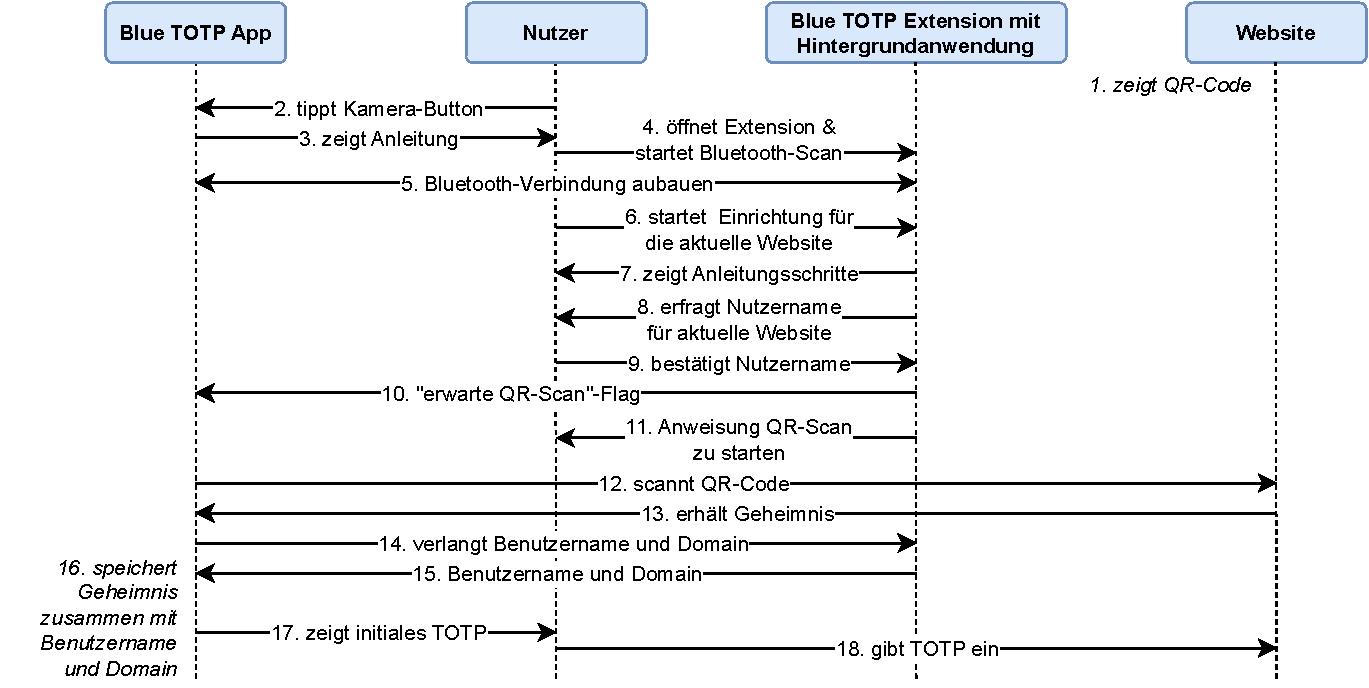
\includegraphics[width=1\linewidth]{figures/impl/blue_totp_setup.pdf}
    \caption[Einrichtungsprozess des Prototyps Blue TOTP]{Einrichtungsprozess des Prototyps Blue TOTP}
    \label{fig: prototyp kommunikation ablauf einrichtung}
\end{figure}
Die Schritte müssen nicht zwingend in dieser Reihenfolge ablaufen, allerdings 
haben alle Probanden der später vorgestellten Studie diesen Ablauf gewählt. 
Die Ausgangssituation sei, dass der Nutzer bereits die 2FA-Einrichtung auf 
der Website begonnen hat und die Website ihm nun einen QR-Code anzeigt und 
das initiale TOTP verlangt.
\\\\
Der Nutzer sieht den QR-Code und öffnet seine Authenticator-App, also Blue 
TOTP. Diese zeigt rechts unten, wie in Abb. \ref{fig: blue totp app 
screenshot nicht verbunden} zu sehen, einen Button mit einer Kamera als 
Symbol. Nach Antippen des Buttons erscheint eine Anleitung (vergl. 
Abb. \ref{fig: blue totp app screenshot anleitung}. Diese besagt, dass der 
Nutzer Bluetooth aktivieren und die Blue TOTP Chrome Extension öffnen soll. 
Dort folgt er der Benutzeroberfläche, um mit der Extension den Bluetooth-Scan 
zu starten, und stellt die Verbindung zum Smartphone (genauer zur App) her. 
Diese Verbindung ist unsicher, da dies für die Studie nicht von Bedeutung 
ist. In einer realen Anwendung sollte diese Verbindung sicher sein, wie es 
das Konzept vorsieht. Erst, wenn Smartphone und App verbunden sind, kann die 
Einrichtung mittels Blue TOTP in der Extension gestartet werden (vergl. 
Abb. \ref{fig: blue totp ext screenshot verbunden}). Die einzelnen Schritte 
der Anleitungen sind in Anhang \ref{anh: blue totp ext screens} zu sehen. Ziel 
der Anleitung ist es, dem Nutzer allgemeingültig zu erklären, wie er bei 
einer Website zur 2FA-Einrichtung gelangt. Danach erfragt die Extension noch 
den Benutzernamen für die Website. Dieser wird automatisch bei der Anmeldung 
auf der Website erkannt und in diesem Schritt der Anleitung dem Nutzer 
gezeigt. Man kann den Namen ggf. ändern. Dies sollte man aber nur tun, wenn 
nicht der korrekte Nutzername  für die Website vorgeschlagen wird. 
Andernfalls funktioniert der Authentisierungsvorgang später nicht. Nun 
fordert die Extension den Nutzer auf, erneut den Kamera-Button der App 
anzutippen, damit die App den QR-Code scannen kann. Damit die App jetzt nicht 
wieder ihre initiale Anleitung anzeigt, erhält sie von der Extension eine 
Nachricht per Bluetooth, dass der QR-Scan freigegeben ist (Schritt 10). Der 
restliche Verlauf (12. bis 16.) ist identisch mit dem Konzept. Ausnahmen sind 
Schritt 17 und 18. Hier zeigt die App das aktuelle TOTP an, das der Nutzer 
nun ablesen und in die Website eingeben muss. Die Einrichtung ist somit 
abgeschlossen.

\paragraph*{Authentisierung}
\mbox{} \vspace{0.1cm} \\
Der Authentisierungsvorgang unterscheidet sich kaum von der Vorgabe des 
Konzepts. Der Ablauf der Authentisierung ist in Abb. \ref{fig: prototyp 
kommunikation ablauf auth} dargestellt.
\begin{figure}[h]
    \centering
    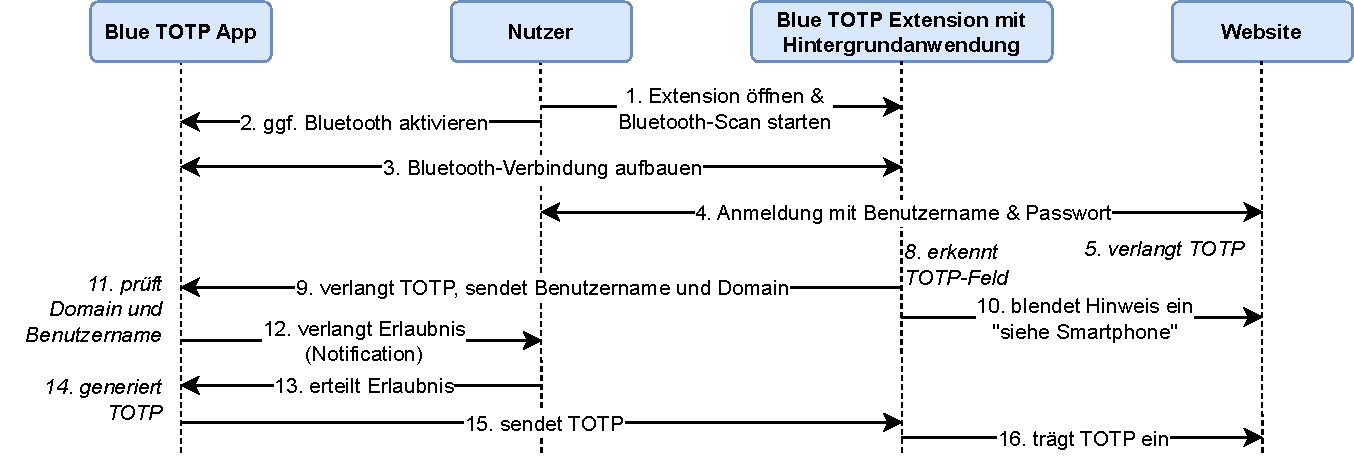
\includegraphics[width=1\linewidth]{figures/impl/blue_totp_login.pdf}
    \caption[Authentisierungsprozess des Prototyps Blue TOTP]{Authentisierungsprozess des Prototyps Blue TOTP}
    \label{fig: prototyp kommunikation ablauf auth}
\end{figure}
Der wesentliche Unterschied zum Konzept ist nur, dass der Nutzer die 
Bluetooth-Verbindung initialisieren muss, indem er die Extension öffnet und 
mit ihr nach seinem Smartphone scannt (Schritt 1). Gegebenenfalls muss er, 
wie in Schritt 2 beschrieben, Bluetooth auf dem Smartphone aktivieren. Die 
App läuft theoretisch immer im Hintergrund. Allerdings kann es je nach 
Android-Version und Konfigurationen vorkommen, dass Android diesen 
Hintergrundprozess beendet, um Energie zu sparen. Dann muss der Nutzer die 
App zusätzlich öffnen. Alle restlichen Schritte sind identisch mit dem 
Konzept bis auf Schritt 10. Hier wird dem Nutzer durch die Extension ein 
Hinweis innerhalb der Website angezeigt, dass er die Notification (aus 
Schritt 12) in seinem Smartphone bestätigen soll. Des Weiteren sei angemerkt, 
dass auch hier die Bluetooth-Verbindung nicht sicher ist, da es für die 
Studie unbedeutend bleibt.
\\\\
Im Fall, dass dem Nutzer kein Bluetooth zur Verfügung steht, gibt es einen 
Fallback in der Blue TOTP App. Jedoch ist er nur experimentell umgesetzt und 
verfügt daher über keinen Phishing-Schutz. Wie beim traditionellen 
TOTP-Verfahren muss der Nutzer das TOTP ablesen und selbst in den Browser 
eintragen.